
%% %%%%%%%%%%%%%%%%%%%%%%%%%%%%%%%%%%%%%%%%%%%%%%%%%
\documentclass[11pt]{article}
\usepackage{UF_FRED_paper_style}
\usepackage{indentfirst}
\usepackage{graphicx}
\captionsetup[figure]{font=scriptsize,labelfont=scriptsize,labelfont=bf}
\captionsetup[table]{font=scriptsize,labelfont=scriptsize,labelfont=bf}

\usepackage{lipsum}  %% Package to create dummy text (comment or erase before start)

%% ===============================================
%% Setting the line spacing (3 options: only pick one)
% \doublespacing
% \singlespacing
\onehalfspacing
%% ===============================================

\setlength{\droptitle}{-5em} %% Don't touch

% %%%%%%%%%%%%%%%%%%%%%%%%%%%%%%%%%%%%%%%%%%%%%%%%%%%%%%%%%%
% SET THE TITLE
% %%%%%%%%%%%%%%%%%%%%%%%%%%%%%%%%%%%%%%%%%%%%%%%%%%%%%%%%%%

% TITLE:
\title{Report on: “A Bayes Factor for Replications of ANOVA Results” by Christopher Harms
}




% AUTHORS:
\author{Jonathon Fleming\\
    {\texttt{jfflemin@ncsu.edu}}  
\and Cole Dunbar\\
    {\texttt{cadunba2@ncsu.edu}} 
\and Tharun Polamarasetty\\
    {\texttt{tpolama@ncsu.edu}}
}
% DATE:
\date{\today}
\begin{document}
\maketitle
% BODY OF THE DOCUMENT
% %%%%%%%%%%%%%%%%%%%%%%%%%%%%%%%%%%%%%%%%%%%%%%%%%%%%%%%%%%
% %%%%%%%%%%%%%%%%%%%%%%%%%%%%%%%%%%%%%%%%%%%%%%%%%%%%%%%%%%

% --------------------
\section{Motivation}
% --------------------

The “replication crisis” has been an issue in psychological studies done in recent years. After completing a replication attempt for an original study, the question comes into play of whether or not the replication study successfully replicated the original study. Previous ideas stated that if both studies are significant and show effects in the same direction, the replication is deemed successful. However, if a significant effect is seen in the original study whereas the effect is non-significant in the replication study, the replication is considered to be failed. This idea, however, leads to misinterpretations, especially in the case of non-significant replications, as the difference between the two results is not tested to see whether it was itself significant. Furthermore, uncertainty is not taken into account with p-values, thus leading to misinterpretations and incorrect assumptions in scientific studies.  

Previous methods to overcome the problems with comparing studies using p-values have been used, one of the more common methods being confidence intervals. After creating a confidence interval (often 95\%), for the original studies effect, a researcher could run a replication study and check to see if the resulting effect falls within the original studies' confidence interval. Although confidence intervals account for the uncertainty that p-values fail to account for, they often lead to misinterpretation. Furthermore, confidence interval width is reliant on sample size and thus the power of the test. It is often the case in psychological studies that power is low, which results in confidence intervals being generally wide for original studies. This causes sensible comparisons of studies to be hard to make, as having a wide interval leads to suggesting a replication study successfully replicated an original study when in fact the replication was not successful.

In recent years scientists have sought to solve this problem by switching from Frequentist methods to Bayesian methods. Verhagen and Wagenmakers proposed a method known as the Replication Bayes factor \citep{Verhagen2014}. This method makes few assumptions about prior beliefs and allows for the testing of the hypothesis that the effect in a replication study is in line with an original study against the hypothesis that there is no effect. This method works well, but can only be applied to t-tests with 1 or 2 samples. Because of this, there is currently not an effective way to study replication tests in which there are 3 or more samples. The limiting factor has always been the loss of directionality when switching from a t-test to an F-test.

In his paper, Harms adapts the Replication Bayes factor model and extends it to F-tests, thus effectively allowing it to be used with any number of groups. His extended model has the same benefits as the t-test model, but with the added benefit of allowing for multiple groups \citep{Harms2019}.


% --------------------
\section{Methodology}
% --------------------

%% Replication Bayes Factor equation for t-test
\begin{equation}
	\label{eq:bf-rep-t}
	\text{B}_{\text{r}0} = \frac{\int t_{df_{\mathrm{rep}}, \delta \sqrt{N_{\mathrm{rep}}}}(t_{\mathrm{rep}}) p(\delta | \delta_{\mathrm{orig}}, H_r) \ \mathrm{d}\delta}{t_{df_{\mathrm{rep}}}(t_{\mathrm{rep}})}
\end{equation}
%% Replication Bayes Factor equation for F test
\begin{equation}
	\label{eq:bf-rep-F}
	\text{B}_{\text{r}0} = \frac{\int \! F_{df_{\mathrm{effect}},df_{\mathrm{error}},f^2\cdot N}(F_{\mathrm{rep}}) p(f^2 | Y_{\mathrm{orig}}) \ \mathrm{d}f^2}{F_{df_{\mathrm{effect}},df_{\mathrm{error}}}(F_{\mathrm{rep}})}
\end{equation}

Harms uses many examples and results in his paper to show the benefit of his Replication Bayes factor model over other models. Equation \eqref{eq:bf-rep-t} is the model Verhagen and Wagenmakers used to first calculate the Replication Bayes factor for t-tests \citep{Verhagen2014}. Harms then proposed equation \eqref{eq:bf-rep-F} as an extension of the previous model to calculate the Replication Bayes factor for F-tests \citep{Harms2019}. Throughout the paper, Harms focuses on equation \eqref{eq:bf-rep-F}, but uses equation \eqref{eq:bf-rep-t} as a comparison for the accuracy of his proposed model. Importance sampling was used to estimate the marginal likelihood of both models, which is suggested to be more effective than Monte Carlo methods, especially in extreme cases. In our report, we replicated the three key sections of his paper that we felt were the most relevant to the added benefit of his model. 

In \textit{Simulation 1: Behavior in Different Scenarios}, Harms simulates how the Replication Bayes factor is altered based on various combinations of sample size, effect size, and number of groups. We condensed the number of combinations to make computation time more efficient while still showing the significant results of this section. Six combinations of original and replication sample size were considered \{(10,10), (10,25), (10,50), (25,25), (25,50), (50,50)\}. These combinations were then used to calculate the Replication Bayes factor for all combinations of k =\{2,3,4,5\} and $f^2$ = \{0.00001, 0.15, 0.35\}, where k is the number of groups and $f^2$ is the effect size. The results were then plotted and displayed in \textbf{Figure \ref{fig:1}}.


In \textit{Simulation 3: F-Test for Two Groups}, Harms looks to see if there is any difference in the Replication Bayes factor when using the t-test model vs his F-test model for a study with two independent groups. We again considered a subset of the number of combinations he used. Four combinations of original and replication sample size were considered \{(15,50), (15,100), (50,50), (50,100)\}. These combinations were then used to calculate the Replication Bayes factor using both the t-test and F-test models for all combinations of d = \{0.2, 0.6, 1\} in which d replication is greater than or equal to d original (d is the Cohen’s d factor for effect size) \citep{cohen1988}. This simulation was only run once in his paper, but we scaled the simulation so that in our simulation N=2 instead of N=1. The results were then plotted and displayed in \textbf{Figure \ref{fig:2}}.

In \textit{Example 3}, the Replication Bayes factor for the F-test shows significance, but this significance is incorrect due to the loss of directionality. In this example, an imaginary study is designed with 3 groups of 15 participants where $\mu_1$ = 1.5, $\mu_2$ = 2.2 and $\mu_3$ = 2.9 for the 3 groups respectively. The standard deviation is 1 for all groups. An ANOVA test concludes a significant result, and the resulting effect size is 0.377. For the replication study, 30 participants are assigned to each of the 3 groups and the resulting group means are similar to the original study but in reverse order. An ANOVA test also concludes a significant result, this time with an effect size of 0.175. The Replication Bayes factor is then calculated, and then compared to the results when doing a post-hoc t-test.The means are plotted in \textbf{Figure \ref{fig:3}}, and the t-values and Bayes factors can be found in \textbf{Table \ref{table:1}}.


% --------------------
\section{Major Results}
% --------------------
Our \textit{Simulation 1} results are shown in \textbf{Figure \ref{fig:1}}. The figure shows that a replication sample size larger than the original, as well as a large replication effect size, gives support to the proponent’s position, as the Bayes factor is larger than 1 in these scenarios. Furthermore, a small effect size in both studies leads to a situation in which the proponent’s and skeptic’s positions are very similar, and thus n must be extremely large to notice any difference, as even n = 50 is not enough to see a difference. If the original study has a large effect whereas the replication study has a small effect, then this leads to evidence in favor of the skeptic’s positions. Also, by holding group sizes equal (n), we can see that by increasing group numbers from 2 to 4, we see more significant results. This suggests more groups allows for stronger conclusions since total sample size is higher. 

Results for our \textit{Simulation 3} in \textbf{Figure \ref{fig:2}} show that the resulting Bayes factors are  very close, with only one outlier for one of the replications when n original = 15, n replication = 100, d original = .2, and d replication = 1 (bottom left quadrant). This outlier makes sense, as this value is at the extremes, when both the n and d values between original and replication study are very different. All other times, however, the Bayes factor from the t-test and F-test lead to the same result, with r = 0.956. One significant finding that is not easily visible in the figure is that the Bayes factor for a t-test is about twice the Bayes factor for an F-test on average. This suggests a relationship for Bayes factor t-test to F-test, similar to how F-test is the t-test squared.

Our generated \textit{Example 3} results are shown in \textbf{Table \ref{table:1}} and \textbf{Figure \ref{fig:3}}. \textbf{Table \ref{table:1}} presents the original and replication t-tests as well as the resulting Bayes factor for the comparison of each group. As can be seen, the Bayes factor for group 1 vs group 3 was significant, suggesting that the study was successfully replicated. However, looking at the values we can see they are similar in magnitude but opposite in direction. By plotting the means of the original and replication study (\textbf{Figure \ref{fig:3}}), we can see that the replication study shows the reverse pattern of the original study, and thus should not be concluded as a successful replication. This misconclusion occurs as a result of the loss of directionality when using F-tests. This result shows that the Bayes factor cannot itself be used as a sole method for concluding significance when considering F-tests. The researcher must inspect the data to ensure that the results are not opposite in direction, or must run a post-hoc t-test along with the Bayes factor to see if there is significance. 
\begin{figure}[H]
    \centering
        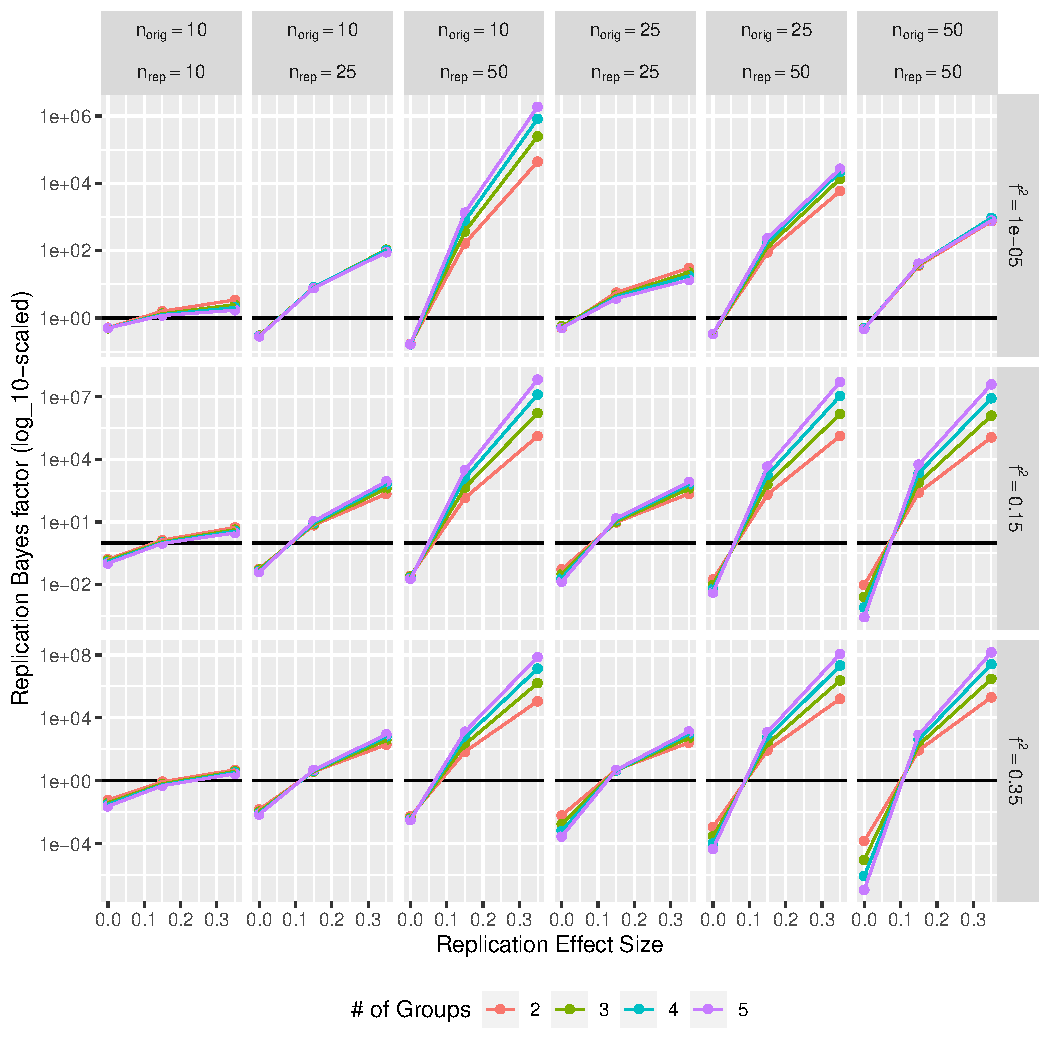
\includegraphics[scale=0.8]{figures/Group_9_Figure_1.pdf}
    \caption{Value of the Replication Bayes factor for F-tests in various scenarios. Columns show sample sizes per group in original and replication study, rows are f2 effect sizes in the original study. Horizontal axes in each plot show f2 effect size in replication study and vertical axes are log10-scaled showing Replication Bayes factor.}  
    \label{fig:1}
\end{figure}
\begin{figure}[H]
    \centering
        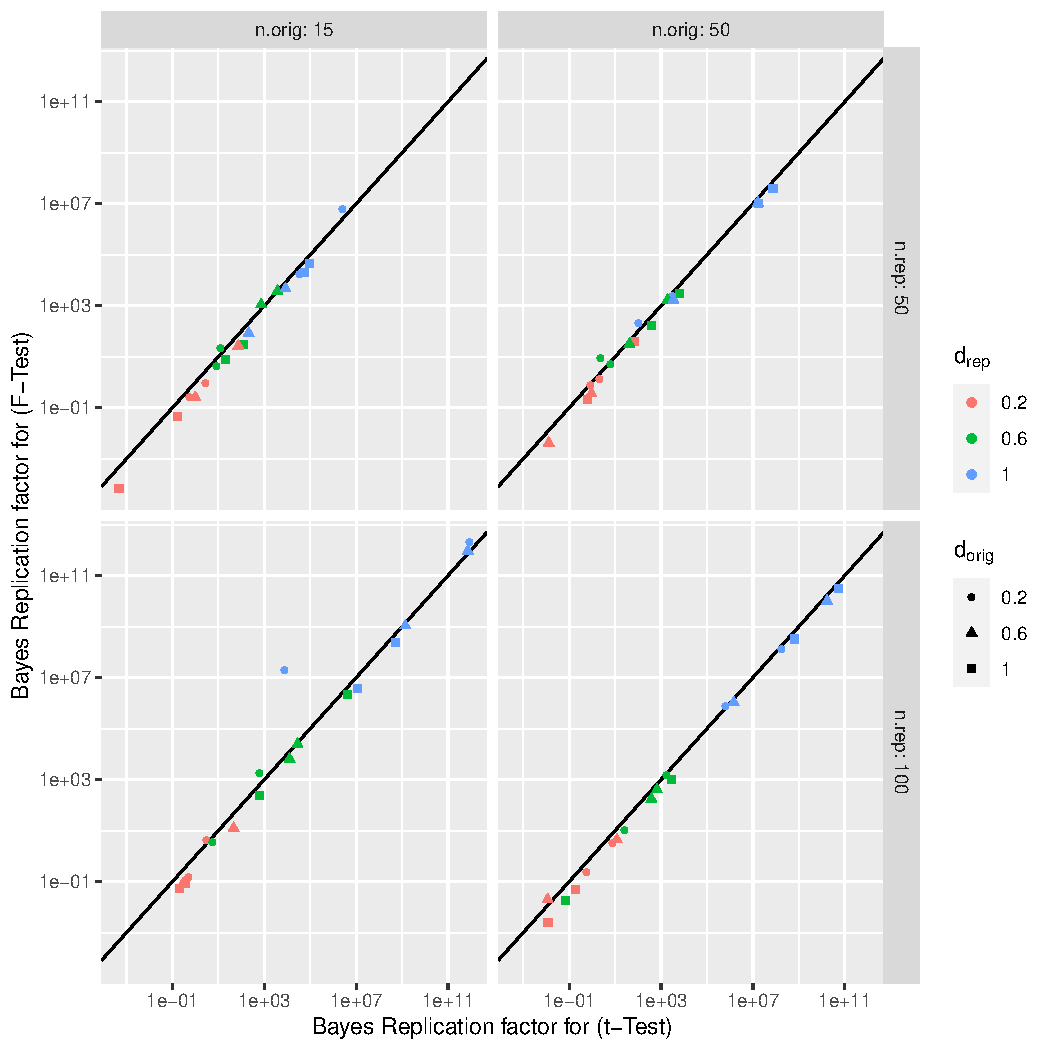
\includegraphics[scale=.9]{figures/Group_9_Figure_2.pdf}
    \caption{Comparison of Replication Bayes factors for t-test and F-test for two independent groups. The solid black line represents equality between the two tests.}
    \label{fig:2}
\end{figure}
\begin{table}[H]
    \centering
        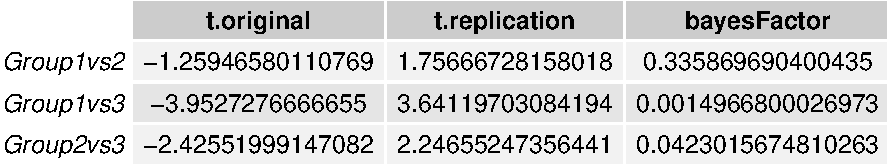
\includegraphics[scale=.8]{figures/Group_9_Table_1_cropped.pdf}
    \caption{Table of t-values and Replication Bayes factor for all pairwise comparisons of groups.}
    \label{table:1}
\end{table}
\begin{figure}[H]
    \centering
        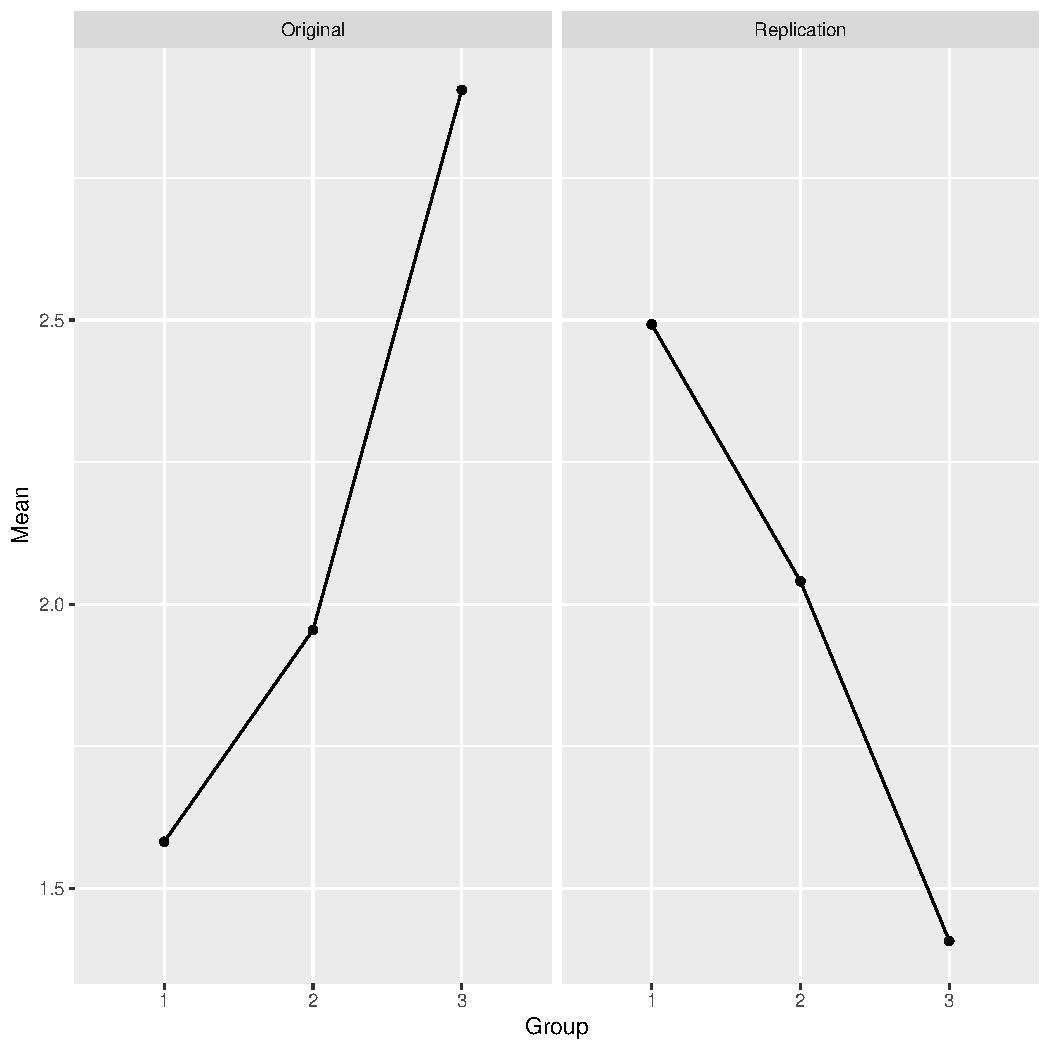
\includegraphics[scale=.7]{figures/Group_9_Figure_3.pdf}
    \caption{Plot of means for original and replication studies.}
    \label{fig:3}
\end{figure}
% --------------------
\section{Conclusions}
% --------------------

This study shows that the Replication Bayes factor using F-tests proposed by Harms is an effective, alternative way to determine the success of a replication study. It produces the same results as the t-test method proposed by Verhagen and Wagenmakers when considering studies with two groups, but it also can be extended to 3 or more groups whereas previous methods could not. The F-test method, however, cannot be the sole judgement of significance for whether or not a replication was successful. Due to the loss of directionality in F-tests, the Bayes factor must be considered alongside the inspection of the data to ensure that the original and replication studies are not opposite in direction. This raises the question of whether or not the method can be improved, or if a new method can be proposed, that is as accurate as Harm’s but does not suffer from the loss of directionality that his method does. Furthermore, the question can arise of what occurs when the samples do not follow a normal distribution. The F-test requires normality in the samples, and it would be useful to inspect the qqplots of the data to see how the Bayes factor could be affected if the samples being used do not adhere to this assumption. 

% %%%%%%%%%%%%%%%%%%%%%%%%%%%%%%%%%%%%%%%%%%%%%%%%%%%%%%%%%%
% %%%%%%%%%%%%%%%%%%%%%%%%%%%%%%%%%%%%%%%%%%%%%%%%%%%%%%%%%%
% REFERENCES SECTION
% %%%%%%%%%%%%%%%%%%%%%%%%%%%%%%%%%%%%%%%%%%%%%%%%%%%%%%%%%%
% %%%%%%%%%%%%%%%%%%%%%%%%%%%%%%%%%%%%%%%%%%%%%%%%%%%%%%%%%%
\medskip

\bibliography{references.bib} 

\newpage

% %%%%%%%%%%%%%%%%%%%%%%%%%%%%%%%%%%%%%%%%%%%%%%%%%%%%%%%%%%
% %%%%%%%%%%%%%%%%%%%%%%%%%%%%%%%%%%%%%%%%%%%%%%%%%%%%%%%%%%
% TABLES
% %%%%%%%%%%%%%%%%%%%%%%%%%%%%%%%%%%%%%%%%%%%%%%%%%%%%%%%%%%
% %%%%%%%%%%%%%%%%%%%%%%%%%%%%%%%%%%%%%%%%%%%%%%%%%%%%%%%%%%



% %%%%%%%%%%%%%%%%%%%%%%%%%%%%%%%%%%%%%%%%%%%%%%%%%%%%%%%%%%
% %%%%%%%%%%%%%%%%%%%%%%%%%%%%%%%%%%%%%%%%%%%%%%%%%%%%%%%%%%
% FIGURES
% %%%%%%%%%%%%%%%%%%%%%%%%%%%%%%%%%%%%%%%%%%%%%%%%%%%%%%%%%%
% %%%%%%%%%%%%%%%%%%%%%%%%%%%%%%%%%%%%%%%%%%%%%%%%%%%%%%%%%%



% ==========================
% ==========================
% ==========================


\end{document}